% Editable article report entrypoint for MediFlow.
%
% This file holds the curated structure of the report. All numbers, tables,
% and figures are pulled in from generated artefacts:
%   ../output/generated/   LaTeX snippets (tables, macros, interpretation text)
%   ../output/figures/     PNG figures referenced via \graphicspath
%
% Refresh those artefacts before compiling: python -m src.cli analyse --no-compile

\documentclass[11pt,a4paper]{article}
\usepackage[utf8]{inputenc}
\usepackage[T1]{fontenc}
\usepackage{lmodern}
\usepackage[english]{babel}
\usepackage[margin=2.2cm]{geometry}
\usepackage{parskip}
\usepackage{booktabs}
\usepackage{tabularx}
\usepackage{array}
\usepackage{graphicx}
\usepackage{float}
\usepackage[table]{xcolor}
\usepackage{hyperref}
\usepackage{microtype}
\usepackage{caption}
\usepackage{enumitem}
\usepackage[most]{tcolorbox}
\usepackage{fancyhdr}
\usepackage{titlesec}

\definecolor{navy}{RGB}{30,58,95}
\definecolor{headerblue}{RGB}{213,232,240}
\definecolor{notebox}{RGB}{239,246,255}
\definecolor{noteborder}{RGB}{37,99,235}
\definecolor{midgray}{RGB}{107,114,128}
\definecolor{lightgray}{RGB}{245,245,245}

\graphicspath{{../output/figures/}}
% AUTO-GENERATED: document macros
% Refresh with python -m src.cli analyse --no-compile.
\newcommand{\MediFlowBuildDate}{2026-04-15}

\newcommand{\MediFlowBuildTimestamp}{2026-04-15T15:33+02:00}

\newcommand{\MediFlowAnalysisRunLabel}{15 Apr 2026, 15:33}

\newcommand{\MediFlowAutoTag}{[AUTO-GENERATED INTERPRETATION]}

\newcommand{\MediFlowContextPath}{\detokenize{../output/report_context.json}}

\newcommand{\MediFlowGeneratedDir}{\detokenize{../output/generated}}

\newcommand{\MediFlowCareFlowRawRows}{26,179}

\newcommand{\MediFlowMediTrackRawRows}{17,262}

\newcommand{\MediFlowCareFlowRegisteredCases}{26,179}

\newcommand{\MediFlowMediTrackRegisteredCases}{17,165}

\newcommand{\MediFlowCareFlowFinishedCases}{20,456}

\newcommand{\MediFlowMediTrackFinishedCases}{6,123}

\newcommand{\MediFlowCareFlowFinishedPct}{78.1\%}

\newcommand{\MediFlowMediTrackFinishedPct}{35.7\%}

\newcommand{\MediFlowCareFlowOpenPct}{14.1\%}

\newcommand{\MediFlowMediTrackOpenPct}{56.8\%}

\newcommand{\MediFlowCareFlowCancelledPct}{7.7\%}

\newcommand{\MediFlowMediTrackCancelledPct}{7.6\%}

\newcommand{\MediFlowCareFlowMedianDays}{48 days}

\newcommand{\MediFlowMediTrackMedianDays}{57 days}

\newcommand{\MediFlowCareFlowMonthCoverage}{11/12 months}

\newcommand{\MediFlowMediTrackMonthCoverage}{12/12 months}

\newcommand{\MediFlowCareFlowLogicalOrderPct}{99.8\%}

\newcommand{\MediFlowMediTrackLogicalOrderPct}{82.3\%}

\newcommand{\MediFlowCareFlowInversionPct}{0.156\%}

\newcommand{\MediFlowMediTrackInversionPct}{46.0\%}

\newcommand{\MediFlowMediTrackSlashPct}{50.1\%}

\newcommand{\MediFlowMediTrackDashPct}{49.9\%}

\newcommand{\MediFlowMediTrackExactDuplicateRows}{81}

\newcommand{\MediFlowMediTrackCaseRowsRemoved}{16}

\newcommand{\MediFlowCareFlowHovedstadenPct}{93.9\%}

\newcommand{\MediFlowCareFlowSjaellandPct}{5.0\%}

\newcommand{\MediFlowMediTrackHovedstadenPct}{3.5\%}

\newcommand{\MediFlowMediTrackSjaellandPct}{94.6\%}

\newcommand{\MediFlowFoundationPoints}{%
\begin{itemize}
  \item We tested candidate file encodings to find an import setup that preserved the raw values.
  \item We read date columns as text first to find the real source formats before parsing them.
  \item We measured the slash and dash populations to find how mixed the messy date fields were.
  \item We separated exact duplicate rows from duplicate case IDs to find the true case grain.
  \item We marked risky metrics as exploratory to find which comparisons were safe to treat as headline results.
  \item We generated report facts from the script to keep the written outputs aligned with the current run.
\end{itemize}
}

\newcommand{\MediFlowCurrentRunHighlights}{%
\begin{itemize}
  \item CareFlow finished case rate (Completed): 78.1\%
  \item CareFlow open rate at year end: 14.1\%
  \item CareFlow median treatment time: 48 days
  \item MediTrack finished case rate (Done): 35.7\%
  \item MediTrack finish-before-registration rate: 46.0\%
  \item MediTrack RegisteredAt date styles: 50.1\% slash / 49.9\% dash
  \item MediTrack duplicate cleanup in the pipeline: 81 exact rows removed and 16 extra case rows collapsed
\end{itemize}
}

\newcommand{\MediFlowKpiRows}{%
Registered cases (2022) & 26,179 & 17,165 & Case-level comparison \\
Finished cases & 20,456 & 6,123 & Completed vs Done \\
Finished case rate & 78.1\% & 35.7\% & Same concept \\
Open rate & 14.1\% & 56.8\% & MediTrack groups Open, Pending, and In Progress \\
Cancelled rate & 7.7\% & 7.6\% & Comparable \\
Median treatment time & 48 days & 57 days & MediTrack exploratory \\
Finish before registration & 0.156\% & 46.0\% & Date-order check \\
}

\newcommand{\MediFlowScorecardRows}{%
Date format & OK: single YYYYMMDD format & Caution: mixed slash/dash timestamps (50.1\% slash, 49.9\% dash) \\
Parse rate & OK: 100.0\% & OK: 100.0\% \\
Reg <= assign & OK: 99.8\% & Caution: 82.3\% \\
Finish before reg & OK: 0.156\% & Fail: 46.0\% \\
Treatment-time KPI & OK: median 48 d & Exploratory: median 57 d \\
Temporal coverage & Caution: 11/12 months & OK: 12/12 months \\
Duplicates & OK: no duplicate case rows & Fail: 81 exact rows and 16 extra case rows required collapse \\
}

\newcommand{\MediFlowCareFlowCategoryRows}{%
HOME\_MON & 22.9\% & 78.3\% & 7.5\% \\
SURG\_PRE & 19.9\% & 79.7\% & 6.2\% \\
ACUTE & 14.9\% & 75.5\% & 10.4\% \\
REHAB & 13.8\% & 76.8\% & 9.1\% \\
OUTP\_FUP & 10.7\% & 81.2\% & 4.6\% \\
SURG\_POST & 9.5\% & 73.3\% & 12.6\% \\
DIAG & 8.4\% & 82.5\% & 3.4\% \\
}

\newcommand{\MediFlowMediTrackCategoryRows}{%
Kort Sag & 28.0\% & 37.3\% & 6.0\% \\
Pakke A & 22.1\% & 34.8\% & 8.4\% \\
Pakke B & 17.5\% & 32.8\% & 10.4\% \\
Forlob Y & 12.8\% & 38.8\% & 4.5\% \\
Revurdering & 10.9\% & 30.6\% & 12.6\% \\
Forlob X & 8.7\% & 40.2\% & 3.0\% \\
}

\newcommand{\MediFlowCareFlowRegionRows}{%
Hovedstaden & 93.9\% \\
Sjaelland & 5.0\% \\
Other & 1.1\% \\
}

\newcommand{\MediFlowMediTrackRegionRows}{%
Hovedstaden & 3.5\% \\
Sjaelland & 94.6\% \\
Other & 1.9\% \\
}

\newcommand{\MediFlowAutoExecSummary}{%
CareFlow supports a more direct KPI read in this run: 78.1\% finished, 14.1\% still open, and almost no finish-before-registration cases (0.156\%). MediTrack is still useful for case counts and status mix, but 46.0\% of finished cases fall before registration, so the 57 days treatment-time figure should stay a rough check.
}

\newcommand{\MediFlowAutoQualitySummary}{%
The two datasets needed different cleanup steps before comparison. CareFlow uses one date style and does not need case-level deduplication. MediTrack needed two extra checks: parsing mixed RegisteredAt date styles (50.1\% slash / 49.9\% dash) and collapsing 81 exact duplicate rows plus 16 extra RefNo rows to case level. That makes the status and volume comparisons stronger than the treatment-time comparison.
}

\newcommand{\MediFlowAutoGeoSummary}{%
CareFlow mostly uses Hovedstaden postcodes (93.9\%) with a smaller Sjaelland share (5.0\%). MediTrack mostly uses Sjaelland postcodes (94.6\%) with some Hovedstaden spillover (3.5\%). The postcode pools are synthetic and were chosen for readable visual separation, not to describe real regional activity.
}


\pagestyle{fancy}
\fancyhf{}
\fancyhead[L]{\small\color{midgray}MediFlow report}
\fancyfoot[R]{\small\color{midgray}\thepage}
\renewcommand{\headrulewidth}{0.4pt}
\renewcommand{\footrulewidth}{0pt}

\titleformat{\section}{\large\bfseries\color{navy}}{}{0em}{}[\color{navy}\titlerule]
\titleformat{\subsection}{\normalsize\bfseries\color{navy}}{}{0em}{}
\titlespacing*{\section}{0pt}{16pt}{8pt}
\titlespacing*{\subsection}{0pt}{10pt}{5pt}
\newcolumntype{Y}{>{\raggedright\arraybackslash}X}

\newtcolorbox{notebox}{
  colback=notebox,
  colframe=noteborder,
  left=8pt,
  right=8pt,
  top=8pt,
  bottom=8pt,
  boxrule=0.5pt,
  arc=2pt
}

\begin{document}

\begin{titlepage}
\centering
\vspace*{3.2cm}
{\Huge\bfseries\color{navy} MediFlow\par}
\vspace{0.7cm}
{\Large Comparing two synthetic healthcare case extracts\par}
\vspace{0.35cm}
{\large CareFlow North and MediTrack East\par}
\vspace{1.8cm}
{\large Analysis report\par}
\vspace{0.35cm}
{\small Analysis run: \MediFlowAnalysisRunLabel\par}
\vfill
{\small This report keeps the exploratory checks visible, but all current numbers and tables come from the analysis pipeline.\par}
\end{titlepage}

\section{Purpose}

This report follows the same structure as the earlier case work that inspired MediFlow. The aim is simple: check what can be compared across two operational systems, show where the data is strong or weak, and build a repeatable workflow that turns those checks into current figures and tables.

The data in this project is synthetic. The workflow is not. The same kinds of problems are kept on purpose: mixed encodings, mixed date formats, duplicate case IDs, uneven month coverage, and fields that look comparable but should still be treated with care.

\begin{notebox}
\textbf{Questions this report answers}
\begin{enumerate}[leftmargin=*, label=\arabic*.]
  \item Can the two systems be compared at all, and at what grain?
  \item Which source is easier to trust for direct KPI use?
  \item What do we need to clean before the numbers are safe to reuse?
  \item Which categories look most standardised and highest-volume?
  \item What extra patterns show up once the cleaning is done?
  \item What should be fixed now, and what should be built next?
\end{enumerate}
\end{notebox}

\section{Data Basis And Method}

\subsection{The two datasets}

The project compares one cleaner system and one messier one.

\renewcommand{\arraystretch}{1.18}
\begin{tabularx}{\textwidth}{>{\bfseries}p{3.7cm}YY}
\toprule
 & CareFlow North & MediTrack East \\
\midrule
Raw rows & \MediFlowCareFlowRawRows & \MediFlowMediTrackRawRows \\
Rows in the 2022 comparison window & \MediFlowCareFlowRegisteredCases & \MediFlowMediTrackRegisteredCases \\
Date style & One stable \texttt{YYYYMMDD} pattern & Mixed slash and dash timestamps \\
Month coverage & \MediFlowCareFlowMonthCoverage & \MediFlowMediTrackMonthCoverage \\
Main strength & Cleaner process fields & Broader category detail \\
Main weakness & December registrations are missing & Dates and case IDs need more cleanup \\
\bottomrule
\end{tabularx}

\medskip
\noindent The comparison window is case registrations in 2022. That is why CareFlow stays at \MediFlowCareFlowRegisteredCases\ rows after cleaning, while MediTrack comes down from \MediFlowMediTrackRawRows\ raw rows to \MediFlowMediTrackRegisteredCases\ case-level 2022 rows.

\subsection{Method}

\begin{enumerate}[leftmargin=*, label=\arabic*.]
  \item Read the files safely, including encoding checks.
  \item Keep date columns as text first and inspect the raw formats.
  \item Parse dates only after the actual source patterns are clear.
  \item Separate exact row duplicates from duplicate case IDs.
  \item Mark treatment-time metrics as robust or exploratory before plotting them.
  \item Generate figures, tables, and export files from the same pipeline run.
\end{enumerate}

\subsection{What can be compared?}

The systems do \emph{not} support a row-by-row join. They do support a useful case-level comparison because the same business ideas appear in both sources.

\renewcommand{\arraystretch}{1.18}
\begin{tabularx}{\textwidth}{p{4.2cm}p{3.0cm}p{3.0cm}X}
\toprule
Shared idea & CareFlow North & MediTrack East & Use in this report \\
\midrule
Case reference & \texttt{CARE\_REF} & \texttt{RefNo} & Same case grain idea, but not a shared key \\
Registration date & \texttt{DT\_REG} & \texttt{RegisteredAt} & Safe for year and month comparisons \\
Assignment date & \texttt{DT\_ALLOC} & \texttt{AssignedOn} & Safe for order checks \\
Cancelled date & \texttt{DT\_ABORT} & \texttt{CancelledOn} & Safe for cancellation-rate comparison \\
Pathway start & \texttt{DT\_OPEN} & \texttt{StartPathway} & Useful context, not the main KPI basis \\
Finished date idea & \texttt{max(DT\_END, DT\_CLOSE)} & \texttt{FinishedAt} & Comparable in concept, but weaker on the MediTrack side \\
Geography proxy & \texttt{ZIP\_PAT} & \texttt{PostalArea} & Used for map views only \\
Category field & \texttt{TRACK} & \texttt{CareGroup} & Used for category-pattern analysis \\
\bottomrule
\end{tabularx}

\begin{notebox}
\textbf{Bottom line} The project compares the two systems at case level and on shared concepts. It does not pretend they are the same source or that every KPI is equally strong in both.
\end{notebox}

\section{Data Quality}

The two systems need different kinds of help before they can sit in the same report. CareFlow is easier to parse and easier to trust for direct KPI work. MediTrack gives richer category patterns, but the pipeline has to do more validation first.

\subsection{Comparative overview}

% AUTO-GENERATED: data-quality scorecard table
% Refresh with python -m src.cli analyse --no-compile.
% AUTO-GENERATED SCORECARD TABLE
\begin{tabularx}{\textwidth}{>{\raggedright\arraybackslash}p{2.8cm} X X}
\toprule
Dimension & CareFlow North & MediTrack East \\
\midrule
\MediFlowScorecardRows
\bottomrule
\end{tabularx}


\begin{figure}[H]
\centering
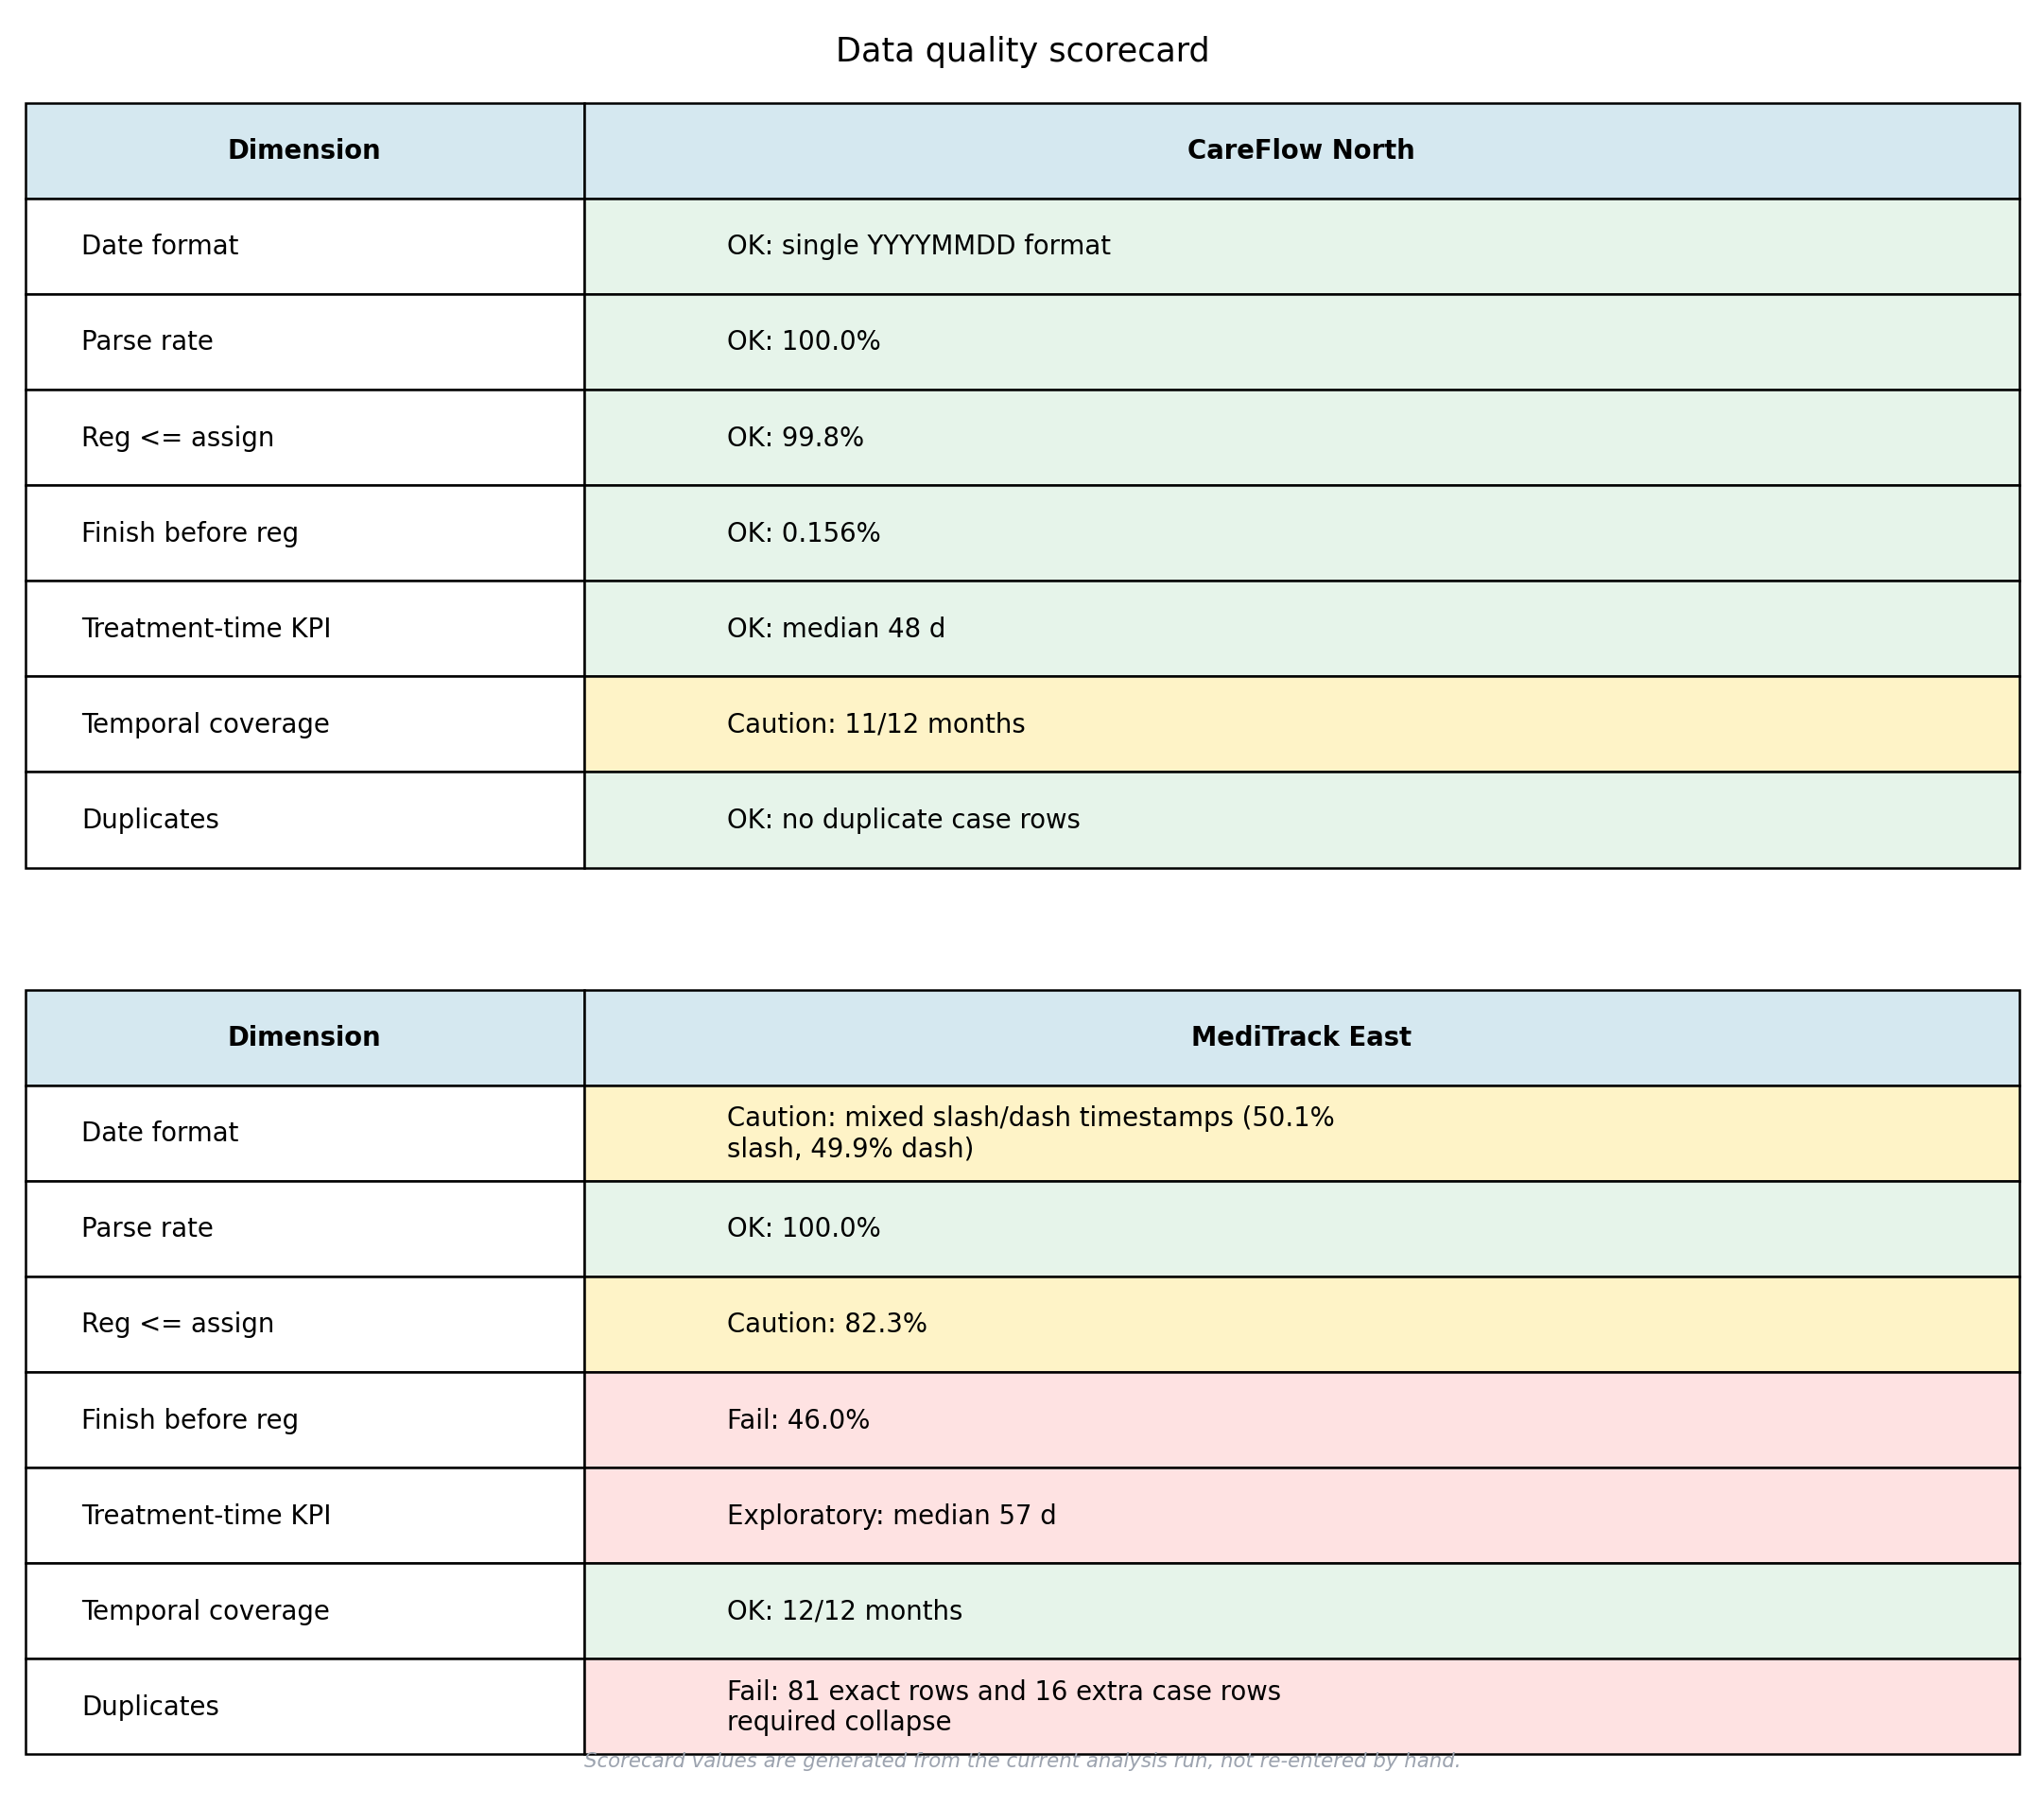
\includegraphics[width=0.96\textwidth]{data_quality_scorecard.png}
\caption{Data-quality scorecard figure generated from the current run.}
\end{figure}

\begin{figure}[H]
\centering
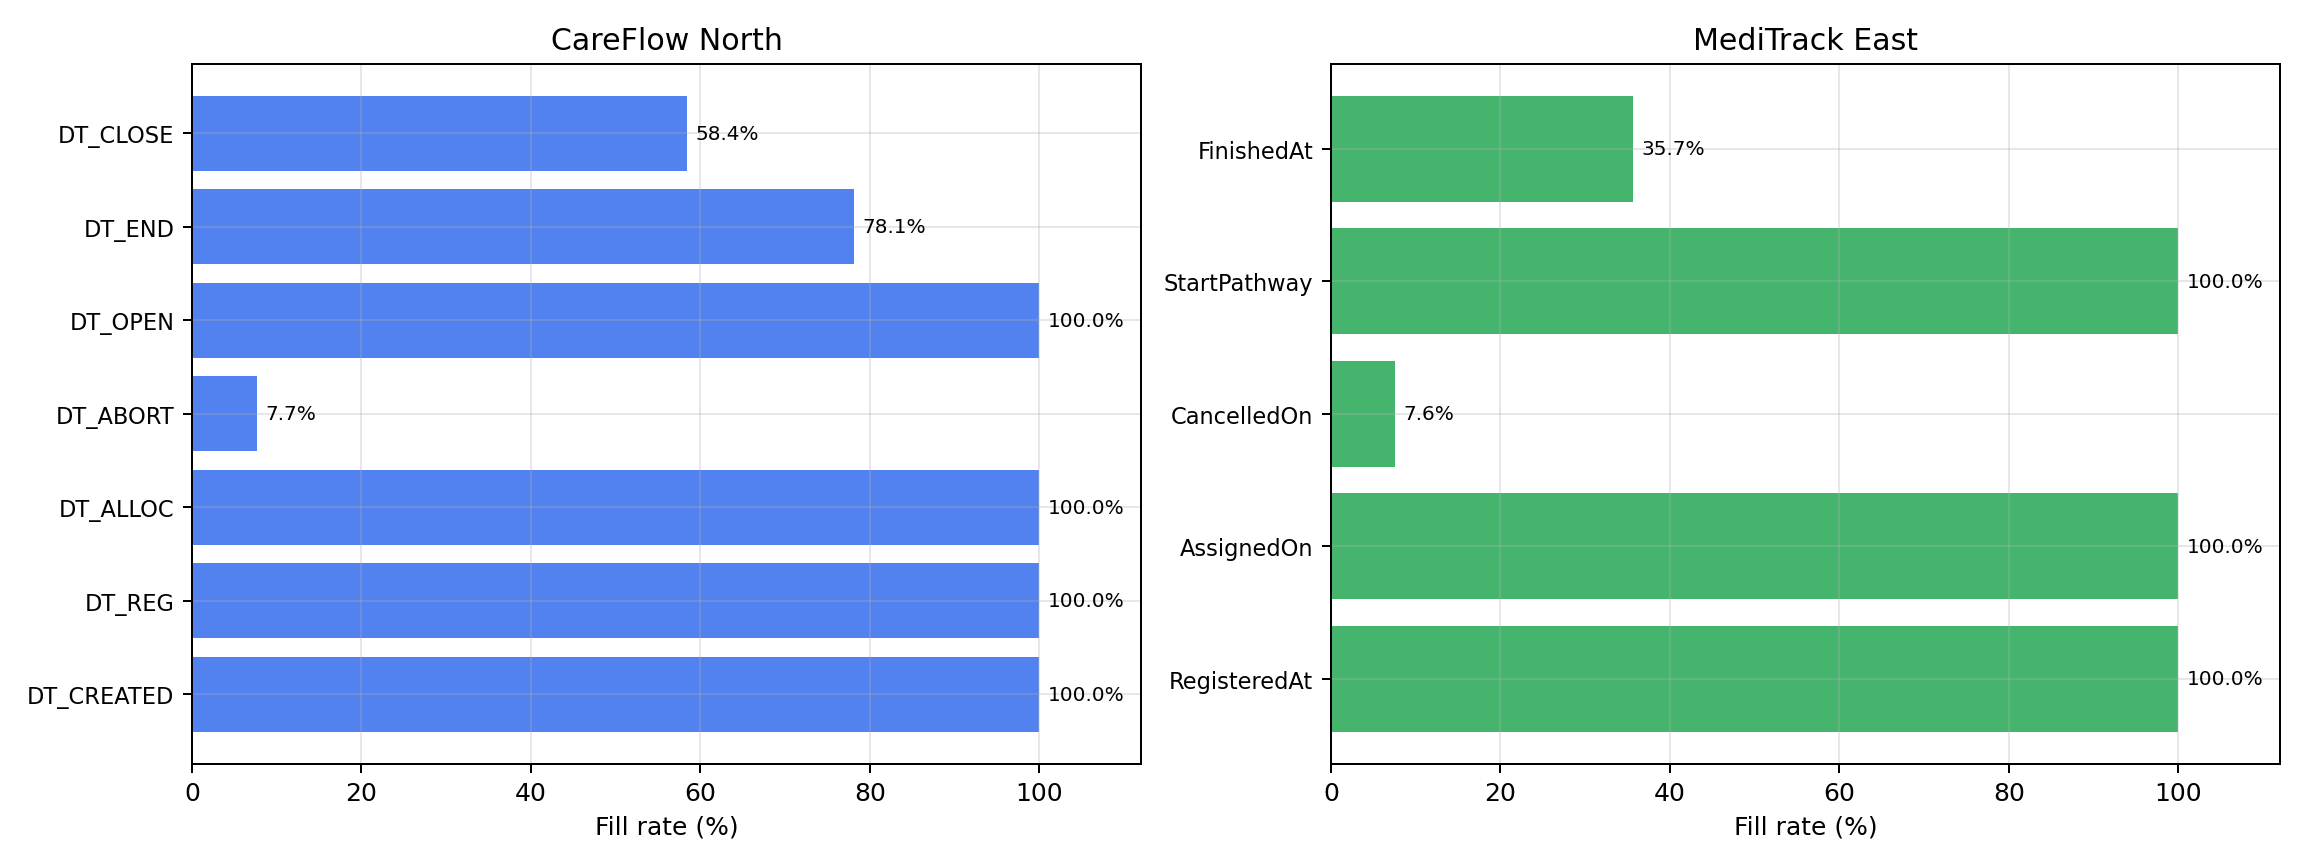
\includegraphics[width=0.96\textwidth]{missing_date_fields.png}
\caption{Date-field completeness. This is useful because a clean format still does not guarantee a complete process trace.}
\end{figure}

\subsection{CareFlow: more consistent, but not complete}

CareFlow is the easier source to work with. It keeps one date style, has almost no finish-before-registration cases (\MediFlowCareFlowInversionPct), and supports a direct finished-case rate of \MediFlowCareFlowFinishedPct.

The main weakness is scope, not parsing. CareFlow only covers \MediFlowCareFlowMonthCoverage, so the year view is intentionally incomplete. It also keeps \texttt{DT\_CREATED} as an older administrative timestamp, which is why the clean system still shows pre-2022 dates in the date-span checks.

\subsection{MediTrack: fuller year, messier dates}

MediTrack covers \MediFlowMediTrackMonthCoverage, but it needs more cleanup before the KPIs make sense. The \texttt{RegisteredAt} field splits almost exactly in half between slash and dash styles (\MediFlowMediTrackSlashPct\ slash / \MediFlowMediTrackDashPct\ dash). The pipeline also removes \MediFlowMediTrackExactDuplicateRows\ exact duplicate rows and collapses \MediFlowMediTrackCaseRowsRemoved\ extra case rows before the comparison reaches case level.

The important warning is date order. \MediFlowMediTrackInversionPct\ of finished cases still fall before registration, so treatment time stays an exploratory check on the MediTrack side even after parsing succeeds.

\section{Date Cleaning And Excel Formulas}

One reason to keep the exploration visible is that the first useful output in a real project is often not a finished report. It is a small practical fix, like helping a department turn exported date strings into usable dates in Excel.

\subsection{What we checked first}

% AUTO-GENERATED: foundation points
% Refresh with python -m src.cli analyse --no-compile.
\MediFlowFoundationPoints


\subsection{Excel formulas kept as working notes}

% AUTO-GENERATED: Excel date parsing note
% Refresh with python -m src.cli analyse --no-compile.
\noindent A practical part of the original exploration was helping a department turn exported date strings into usable Excel dates before any KPI work could start.

\medskip
\begin{tabularx}{\textwidth}{@{}p{4.0cm}X@{}}
\toprule
\textbf{Pattern} & \textbf{Excel formula used in the exploration} \\
\midrule
Clean export (\texttt{YYYYMMDD}) & \begin{minipage}[t]{\linewidth}
\raggedright\ttfamily\footnotesize
=IF(A2=0,"",DATE(LEFT(TEXT(A2,"00000000"),4),\\
MID(TEXT(A2,"00000000"),5,2),\\
RIGHT(TEXT(A2,"00000000"),2)))
\end{minipage} \\[0.8em]
Mixed export (slash / dash timestamps) & \begin{minipage}[t]{\linewidth}
\raggedright\ttfamily\footnotesize
=IF(A2="","",IF(ISNUMBER(SEARCH("/",A2)),\\
DATE(MID(A2,FIND("/",A2,FIND("/",A2)+1)+1,4),\\
LEFT(A2,FIND("/",A2)-1),\\
MID(A2,FIND("/",A2)+1,FIND("/",A2,FIND("/",A2)+1)-FIND("/",A2)-1)),\\
DATE(RIGHT(LEFT(A2,10),4),MID(A2,4,2),LEFT(A2,2))))
\end{minipage} \\
\bottomrule
\end{tabularx}

\noindent\small\textit{These formulas are kept as documentation of the exploration. The Python pipeline now mirrors the same logic, so Excel is not the source of truth for the final report.}


\subsection{Dates outside the 2022 window}

\begin{figure}[H]
\centering
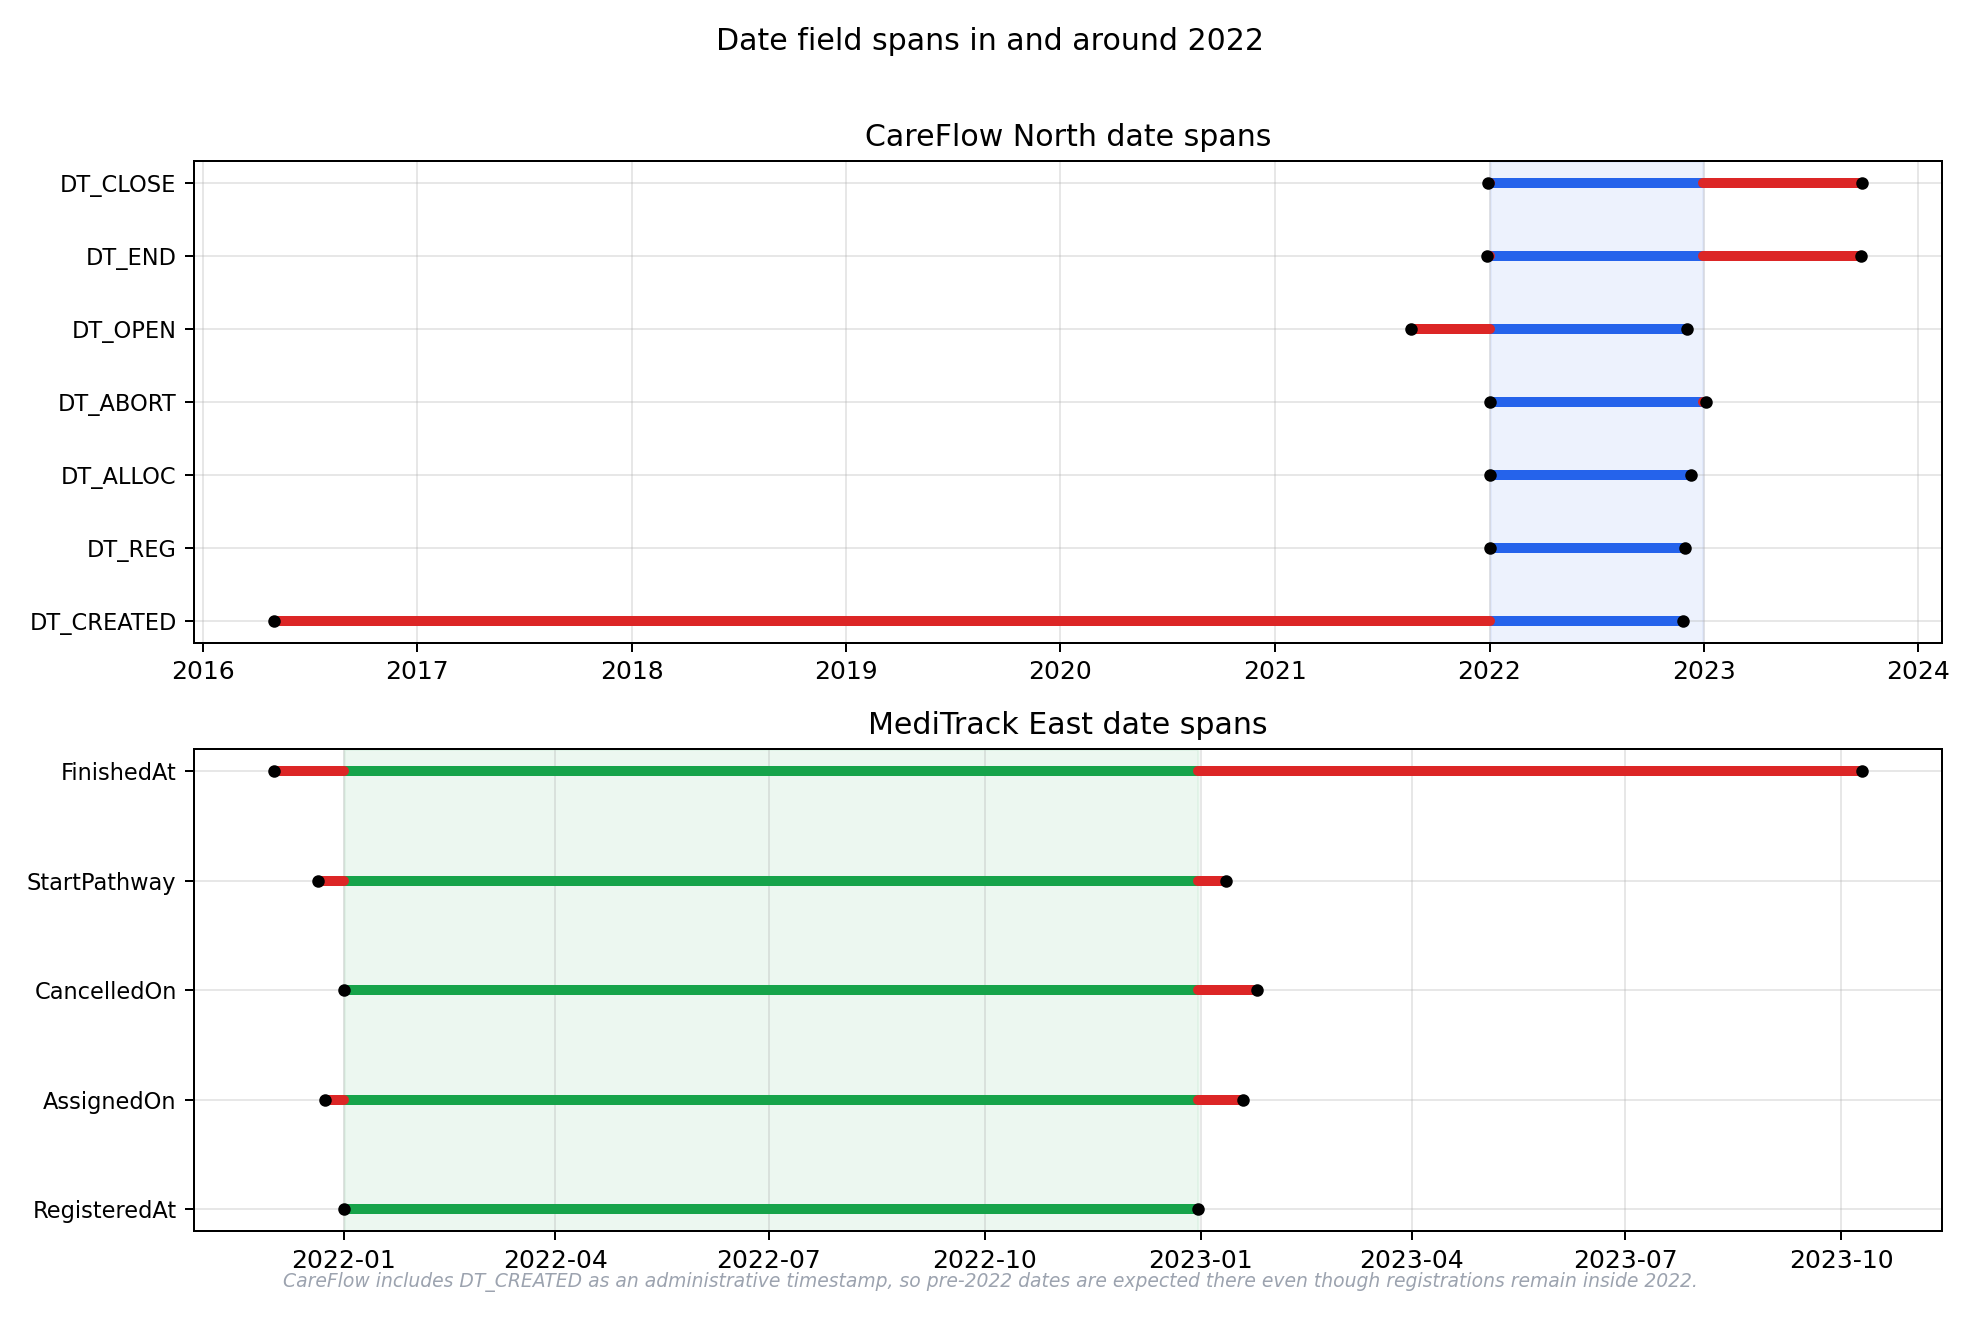
\includegraphics[width=0.96\textwidth]{date_span_outliers.png}
\caption{Date-field spans in and around 2022. CareFlow includes older admin timestamps, while MediTrack shows the effect of mixed process timing and later activity.}
\end{figure}

\section{KPI Overview}

After cleaning, the project can give a stable case-level comparison. The important difference is that not every KPI should be used with the same confidence.

% AUTO-GENERATED: KPI table
% Refresh with python -m src.cli analyse --no-compile.
% AUTO-GENERATED KPI TABLE
{\small
\renewcommand{\arraystretch}{1.12}
\begin{tabularx}{\textwidth}{>{\raggedright\arraybackslash}p{4.0cm} >{\raggedleft\arraybackslash}p{2.2cm} >{\raggedleft\arraybackslash}p{2.2cm} X}
\toprule
Metric & CareFlow North & MediTrack East & Note \\
\midrule
\MediFlowKpiRows
\bottomrule
\end{tabularx}
}


\begin{notebox}
\textbf{\MediFlowAutoTag} % AUTO-GENERATED: report interpretation text
% Refresh with python -m src.cli analyse --no-compile.
% Review this wording if the data changes.
\MediFlowAutoExecSummary

\end{notebox}

\begin{figure}[H]
\centering
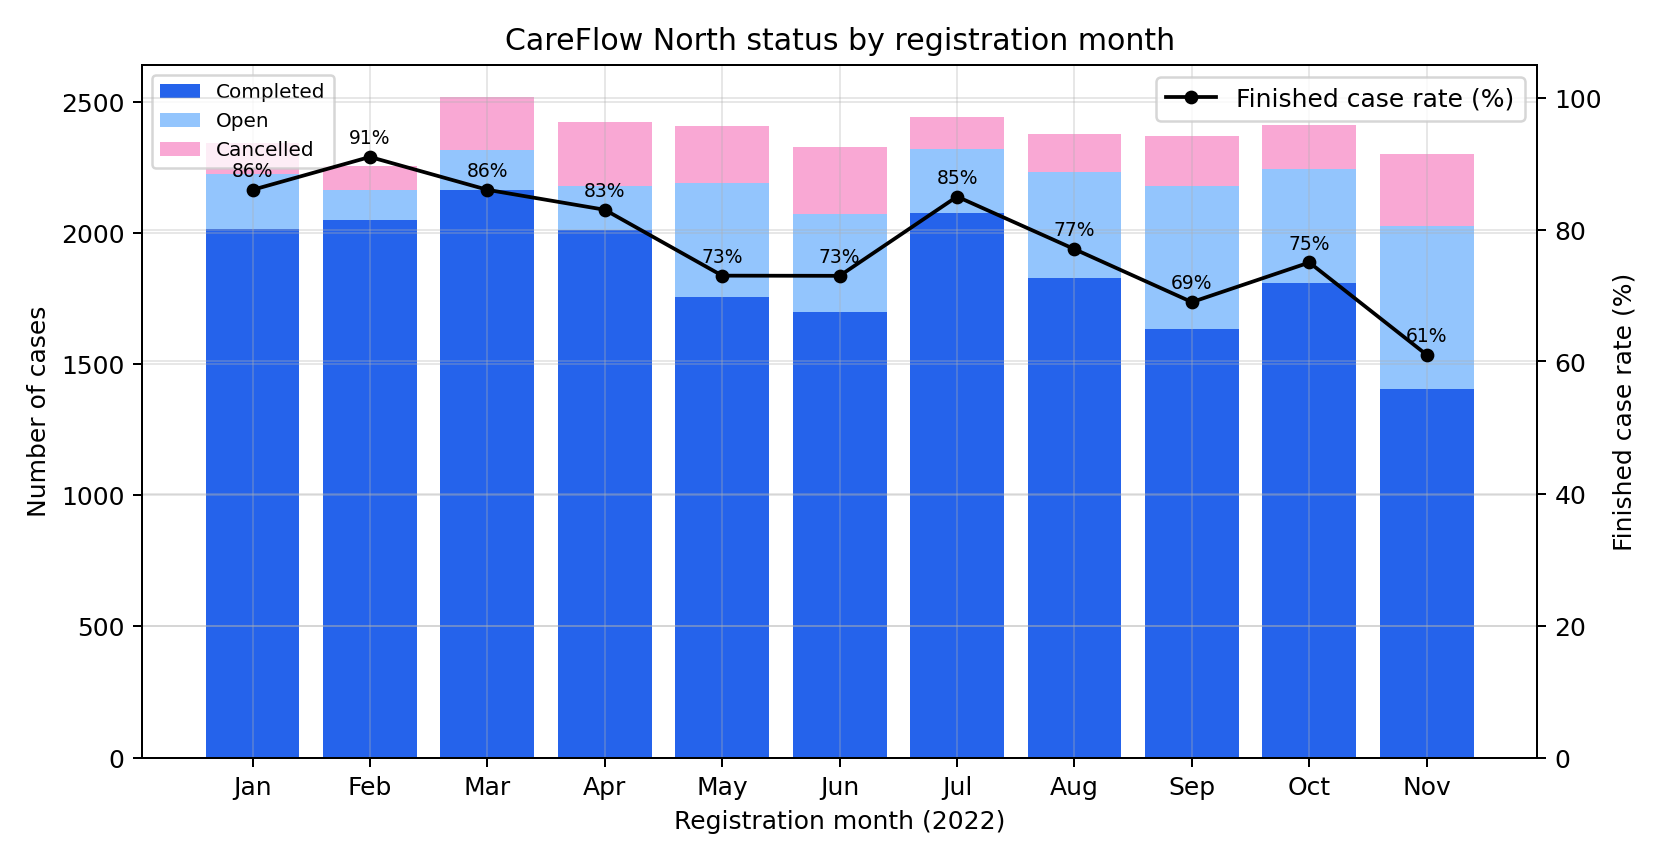
\includegraphics[width=0.96\textwidth]{monthly_status_careflow.png}
\caption{CareFlow monthly status. The clean system still keeps a real backlog and a non-flat cancellation pattern.}
\end{figure}

\begin{figure}[H]
\centering
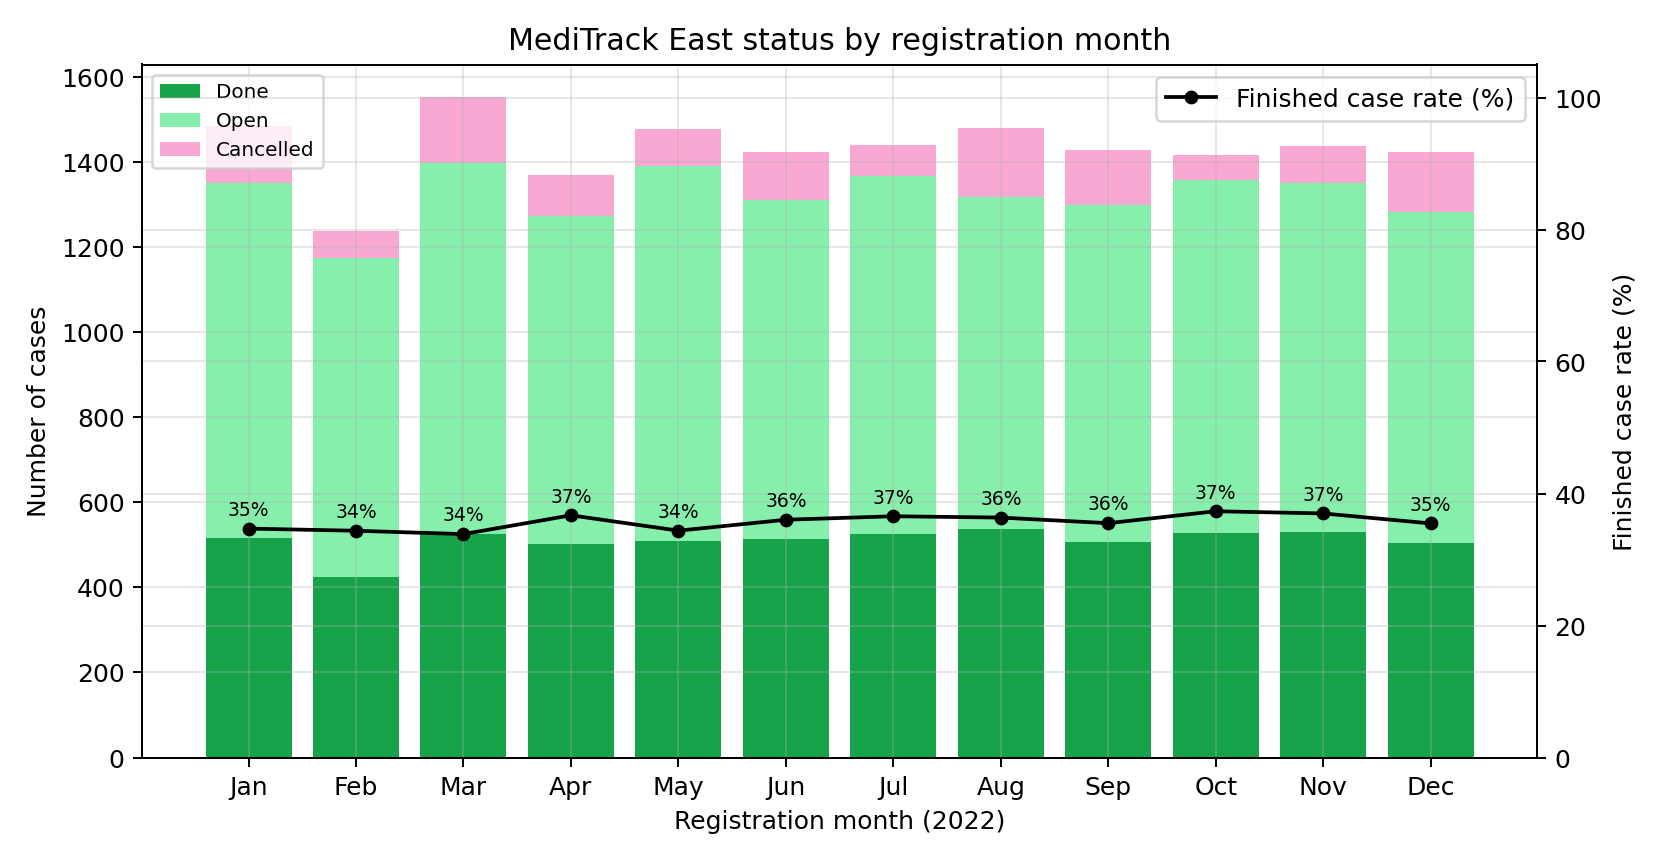
\includegraphics[width=0.96\textwidth]{monthly_status_meditrack.png}
\caption{MediTrack monthly status. Open, pending, and in-progress states are grouped into one open view here so the comparison stays readable.}
\end{figure}

\begin{figure}[H]
\centering
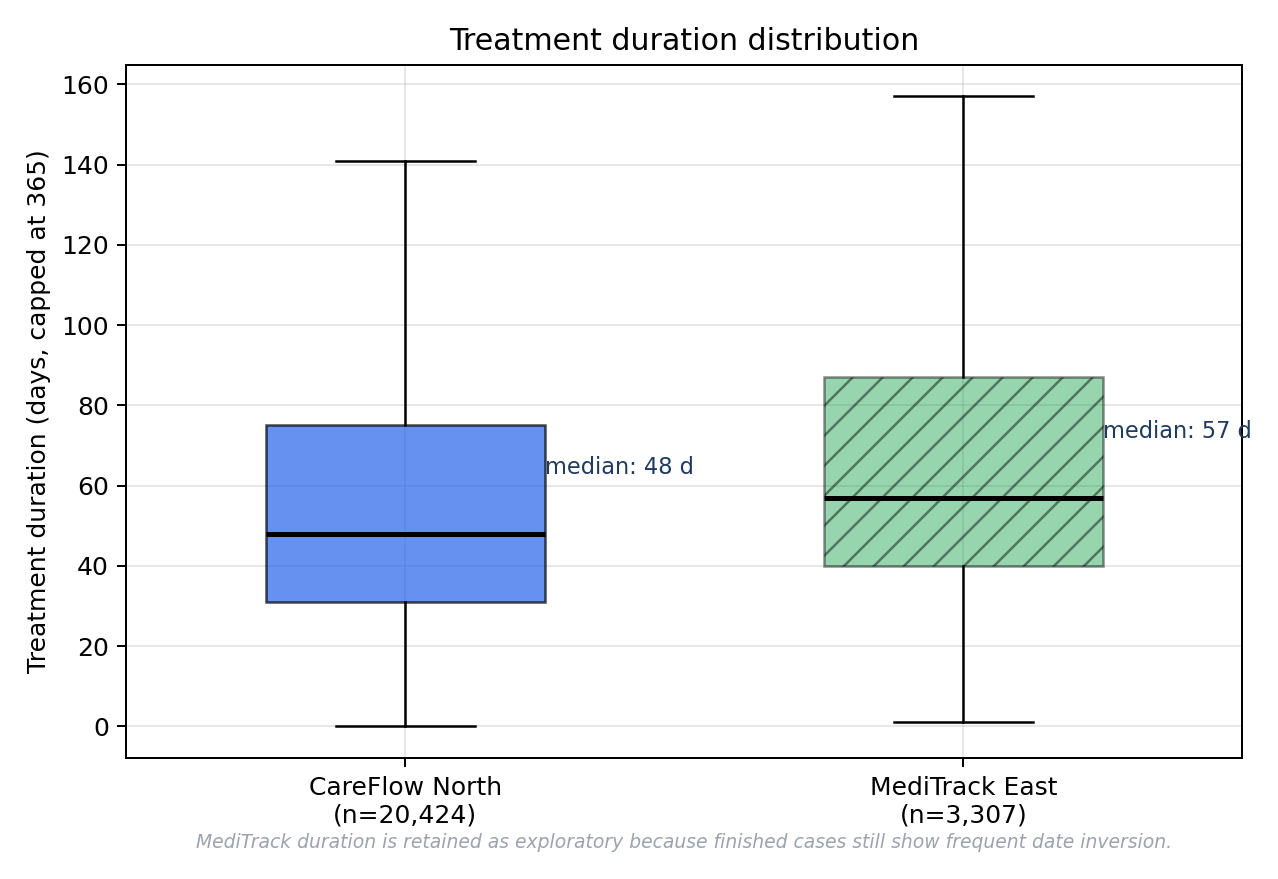
\includegraphics[width=0.96\textwidth]{treatment_duration_boxplot.png}
\caption{Treatment-time distribution for finished cases. CareFlow is suitable for headline use; MediTrack is still shown as an exploratory timing check.}
\end{figure}

\begin{figure}[H]
\centering
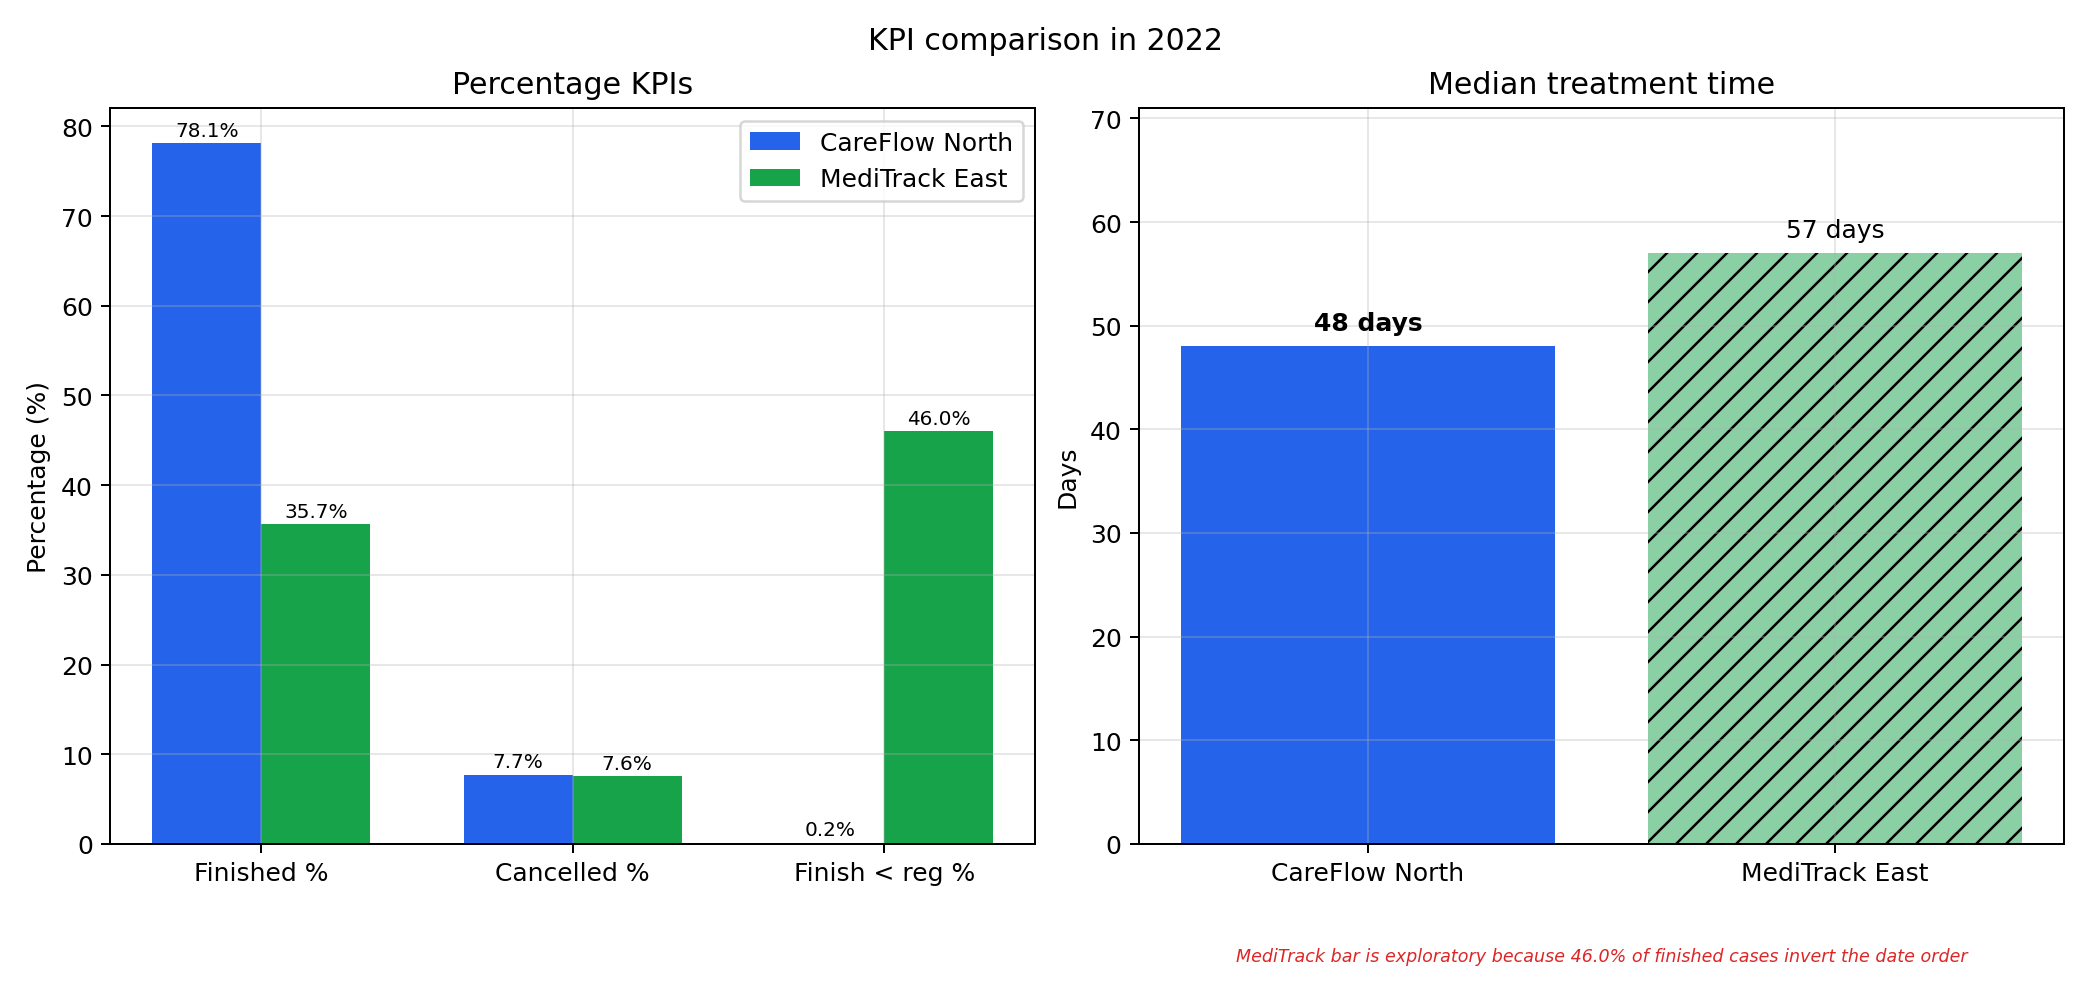
\includegraphics[width=0.96\textwidth]{kpi_comparison.png}
\caption{Compact KPI comparison. The treatment-time panel keeps the MediTrack warning visible.}
\end{figure}

\begin{figure}[H]
\centering
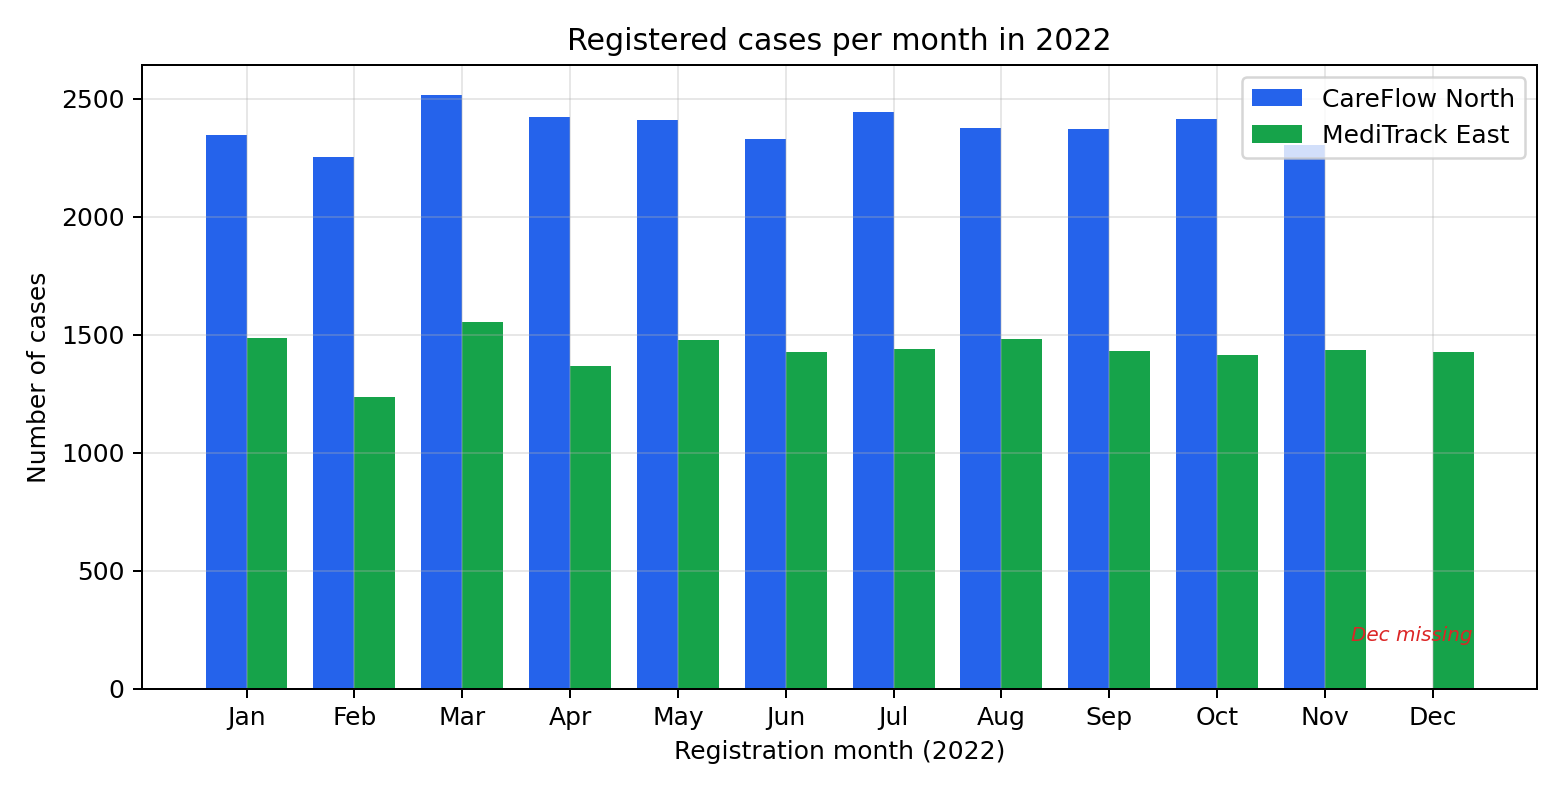
\includegraphics[width=0.96\textwidth]{monthly_volume_2022.png}
\caption{Monthly registration volume. This gives a simple read on the case load across the 2022 study window.}
\end{figure}

\section{Recommendations}

The old case ended with practical recommendations. That structure still works well here.

\subsection{Fix now}

\begin{tabularx}{\textwidth}{p{0.7cm}p{4.2cm}X}
\toprule
\# & Recommendation & Why it matters \\
\midrule
1 & Standardise date exports & MediTrack still mixes slash and dash timestamps in the same field. One clear export pattern would remove a whole layer of cleanup. \\
2 & Define a complete reporting window & CareFlow is clean enough for KPI work, but the missing December cases mean the year view is still incomplete. \\
3 & Keep case grain explicit & The MediTrack comparison only becomes stable after exact row deduplication and case-level collapse on \texttt{RefNo}. \\
\bottomrule
\end{tabularx}

\subsection{Build next}

\begin{tabularx}{\textwidth}{p{0.7cm}p{4.2cm}X}
\toprule
\# & Recommendation & Why it matters \\
\midrule
1 & Publish field definitions with each extract & The report is stronger when field meaning is explicit, especially for finished-date logic. \\
2 & Keep robust and exploratory KPIs separate & That makes it clear which numbers are safe headlines and which are still checks or prompts for follow-up. \\
3 & Automate the intake checks & Encoding checks, date parsing, duplicate handling, month coverage, and report refresh are already scriptable and should stay together. \\
\bottomrule
\end{tabularx}

\section{Category Patterns And Geography}

\subsection{MediTrack category pattern}

The old presentation used category analysis mainly on the messier system, because that was where the readable category labels lived. The same logic still applies here.

% AUTO-GENERATED: MediTrack category table
% Refresh with python -m src.cli analyse --no-compile.
% AUTO-GENERATED CATEGORY TABLE
\begin{tabularx}{\textwidth}{>{\raggedright\arraybackslash}p{4.2cm} >{\raggedleft\arraybackslash}p{2.0cm} >{\raggedleft\arraybackslash}p{2.0cm} >{\raggedleft\arraybackslash}p{2.0cm}}
\toprule
CareGroup & Share & Completed & Cancelled \\
\midrule
\MediFlowMediTrackCategoryRows
\bottomrule
\end{tabularx}


\begin{figure}[H]
\centering
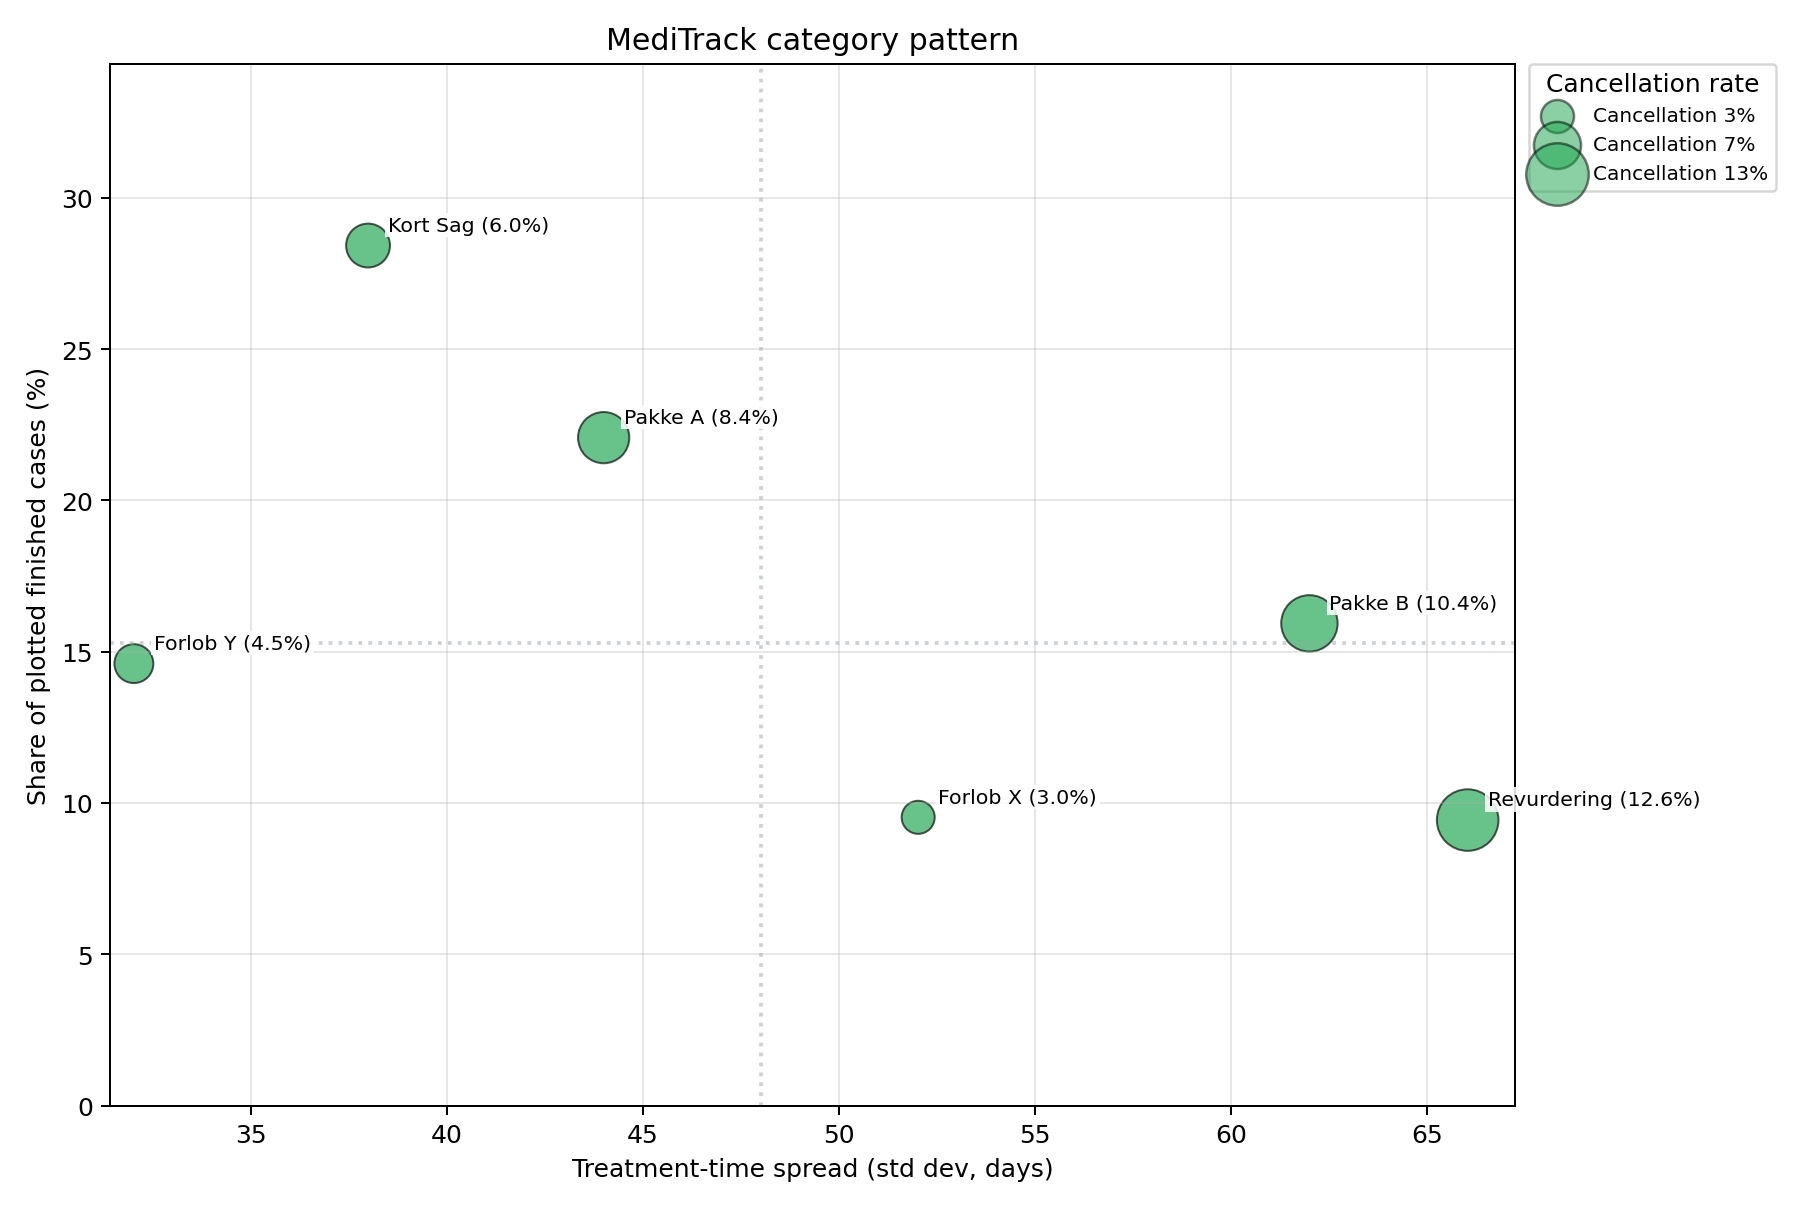
\includegraphics[width=0.9\textwidth]{automation_matrix_meditrack.png}
\caption{MediTrack category pattern. The y-axis now uses relative share, which makes more sense than raw finished counts after cleanup.}
\end{figure}

\subsection{Added view: CareFlow and combined patterns}

MediFlow adds one thing the original case did not have: a matching category view for the cleaner system and a combined view across both systems. That makes it easier to see that category-level spread matters more than a simple clean-versus-messy split.

% AUTO-GENERATED: CareFlow category table
% Refresh with python -m src.cli analyse --no-compile.
% AUTO-GENERATED CATEGORY TABLE
\begin{tabularx}{\textwidth}{>{\raggedright\arraybackslash}p{4.2cm} >{\raggedleft\arraybackslash}p{2.0cm} >{\raggedleft\arraybackslash}p{2.0cm} >{\raggedleft\arraybackslash}p{2.0cm}}
\toprule
TRACK & Share & Completed & Cancelled \\
\midrule
\MediFlowCareFlowCategoryRows
\bottomrule
\end{tabularx}


\begin{figure}[H]
\centering
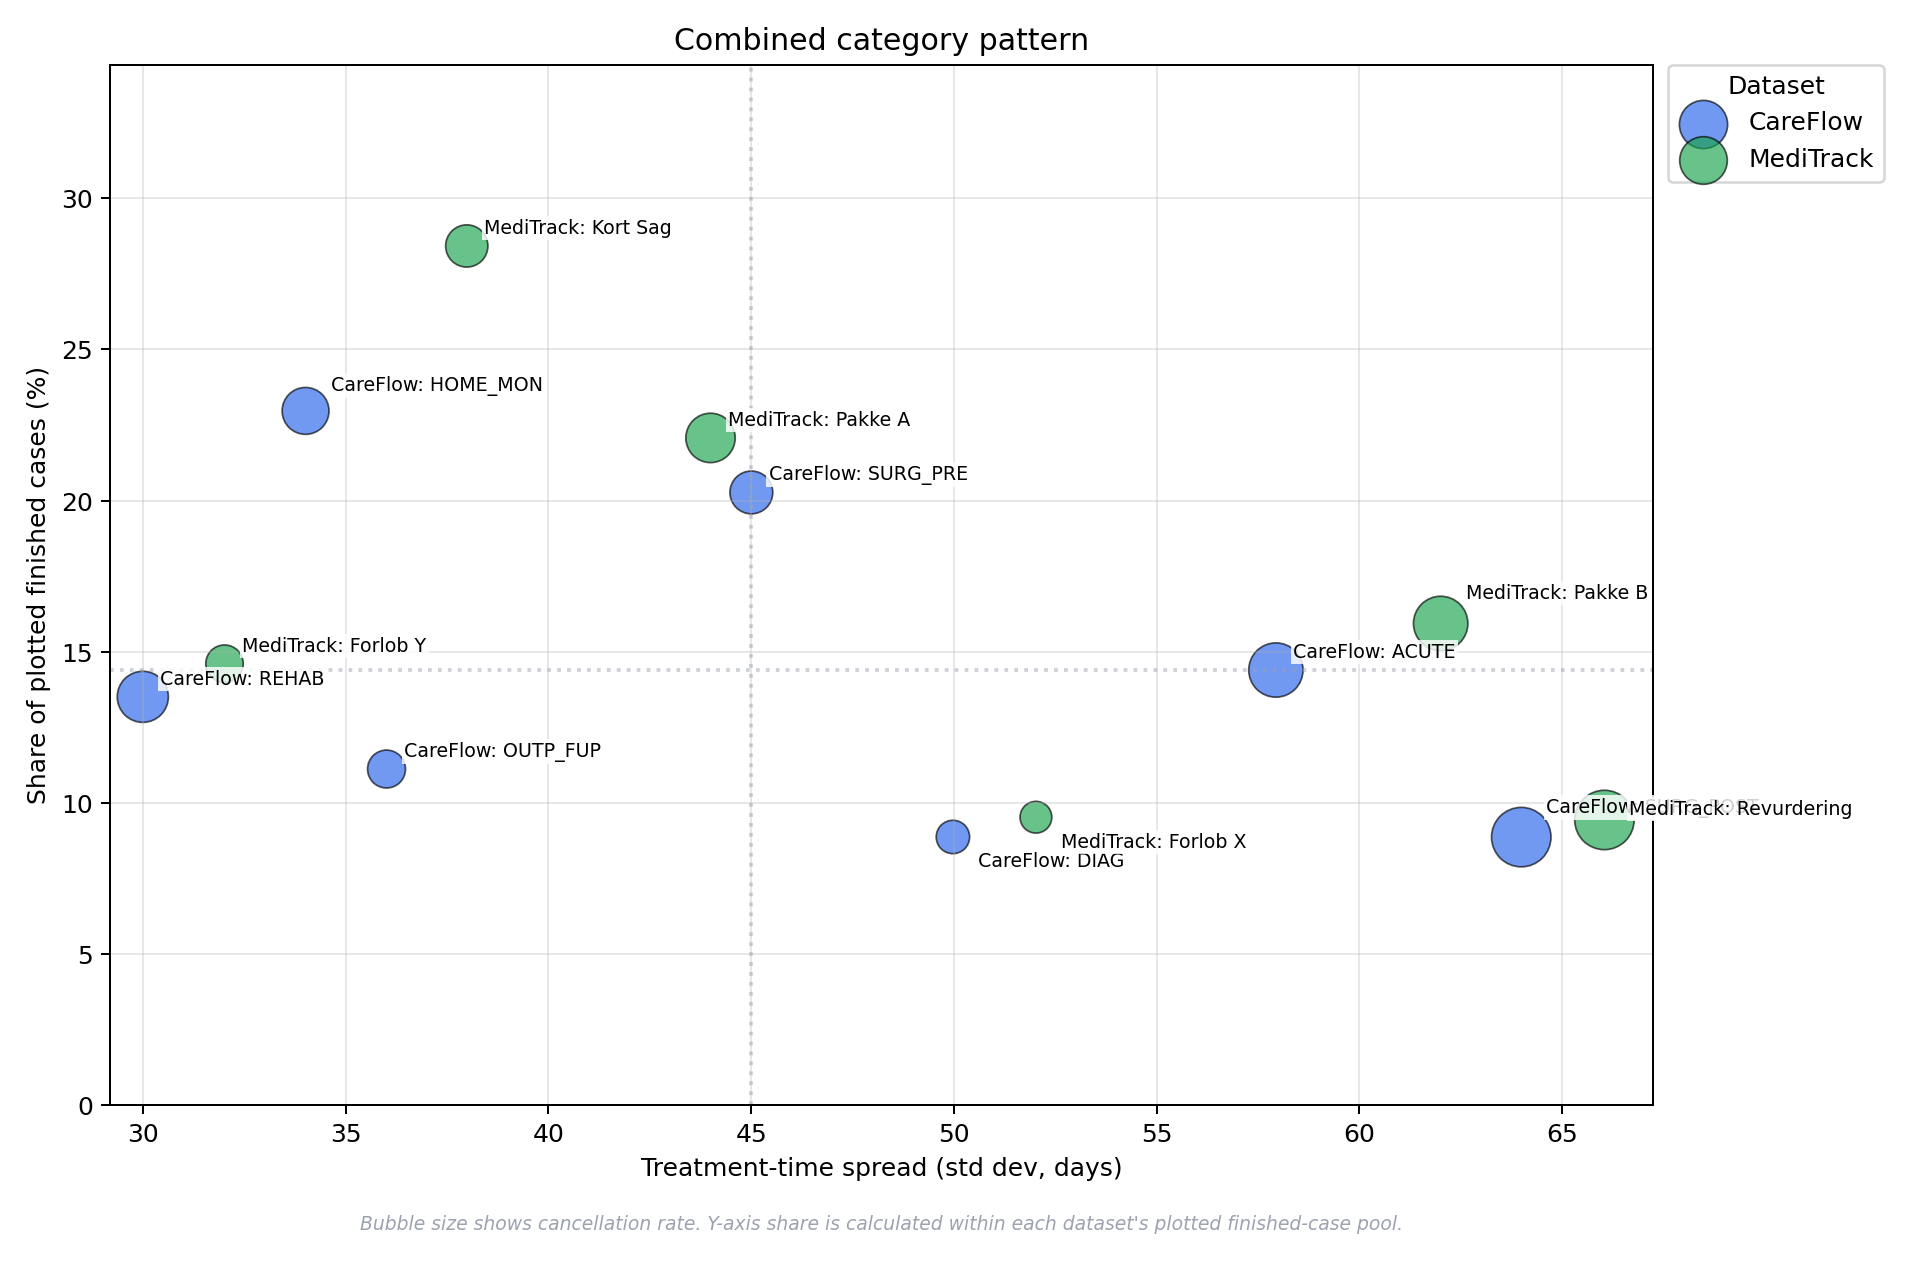
\includegraphics[width=0.9\textwidth]{automation_matrix_combined.png}
\caption{Combined category pattern. This extra view was added in MediFlow to compare category spread and share across the two systems on the same chart.}
\end{figure}

\subsection{Synthetic postcode pools on real geography}

\begin{minipage}[t]{0.48\textwidth}
% AUTO-GENERATED: CareFlow region table
% Refresh with python -m src.cli analyse --no-compile.
% AUTO-GENERATED REGION TABLE
\begin{tabular}{lr}
\toprule
CareFlow pool & Share \\
\midrule
\MediFlowCareFlowRegionRows
\bottomrule
\end{tabular}

\end{minipage}
\hfill
\begin{minipage}[t]{0.48\textwidth}
% AUTO-GENERATED: MediTrack region table
% Refresh with python -m src.cli analyse --no-compile.
% AUTO-GENERATED REGION TABLE
\begin{tabular}{lr}
\toprule
MediTrack pool & Share \\
\midrule
\MediFlowMediTrackRegionRows
\bottomrule
\end{tabular}

\end{minipage}

\begin{figure}[H]
\centering
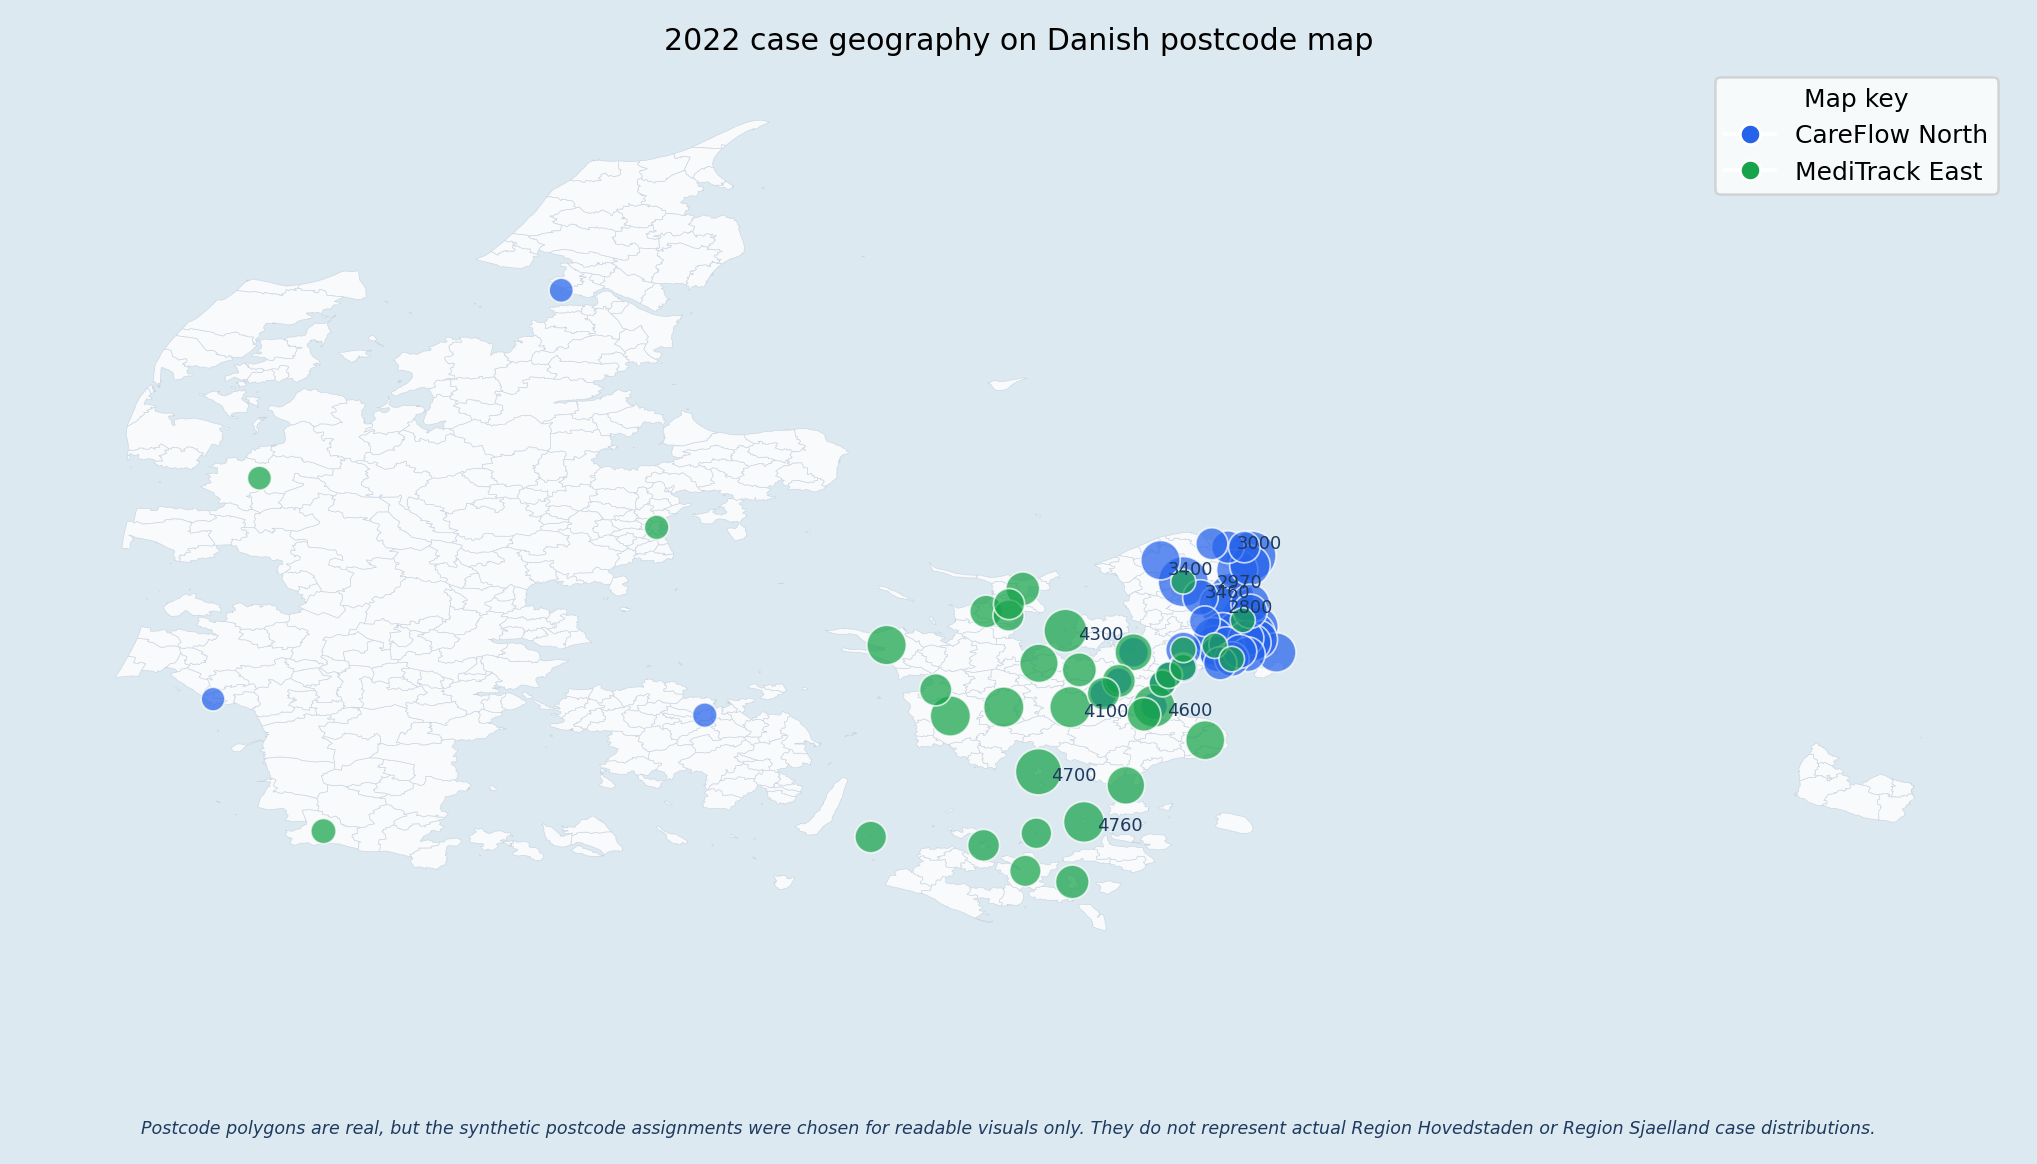
\includegraphics[width=0.96\textwidth]{geo_top15_postalcodes.png}
\caption{Synthetic postcode assignments on real Danish postcode geometry. The shapes are real; the postcode choices are only there to make the visual comparison readable.}
\end{figure}

\begin{notebox}
\textbf{\MediFlowAutoTag} % AUTO-GENERATED: geography interpretation text
% Refresh with python -m src.cli analyse --no-compile.
% Review this wording if the data changes.
\MediFlowAutoGeoSummary

\end{notebox}

\section{Conclusion}

This run supports three plain conclusions:

\begin{enumerate}[leftmargin=*, label=\arabic*.]
  \item The two systems can be compared at case level and on shared concepts, but not by joining rows across systems.
  \item CareFlow is the stronger source for direct KPI reporting, while MediTrack is still better treated as a richer but messier source that needs more caution.
  \item The biggest immediate value is in the data workflow itself: stable import, stable parsing, clear case grain, and report refresh from one pipeline run.
\end{enumerate}

\end{document}
